\begin{surferPage}[Quintic (15 Cusps)]{משטח ממעלה חמישית עם 15 חודים}
  זהו משטח ממעלה חמישית שבו יש $15$ נקודות סינגולריות מסוג $A_2$
    משטח זה, יחד עם מספר משטחים נוספים הקשורים אליו, נכלל
    במאמר שפרסם אוליבר לאבס בשנת 2005.
    חמישה מבין החודים שונים במראה מעשרת החודים האחרים.
    ואכן, חמש נקודות הסינגולריות השונות הן מסוג $A_2^{++}$, ואילו האחרות הן מסוג $A_2^{+-}$ (למידע נוסף
    ראו גלריה על נקודות סינגולריות פשוטות):

     \vspace*{-0.3em}
    \begin{center}
      \begin{tabular}{c@{\qquad}c}
        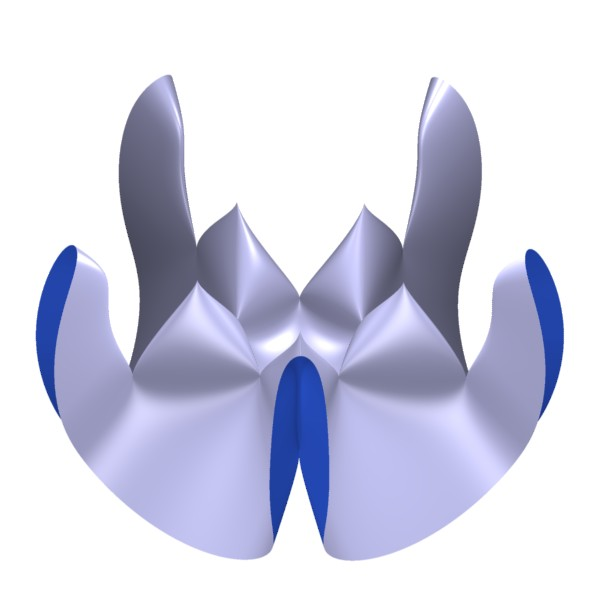
\includegraphics[height=1.2cm]{./../../common/images/dessins_quint_15a2}
        &
        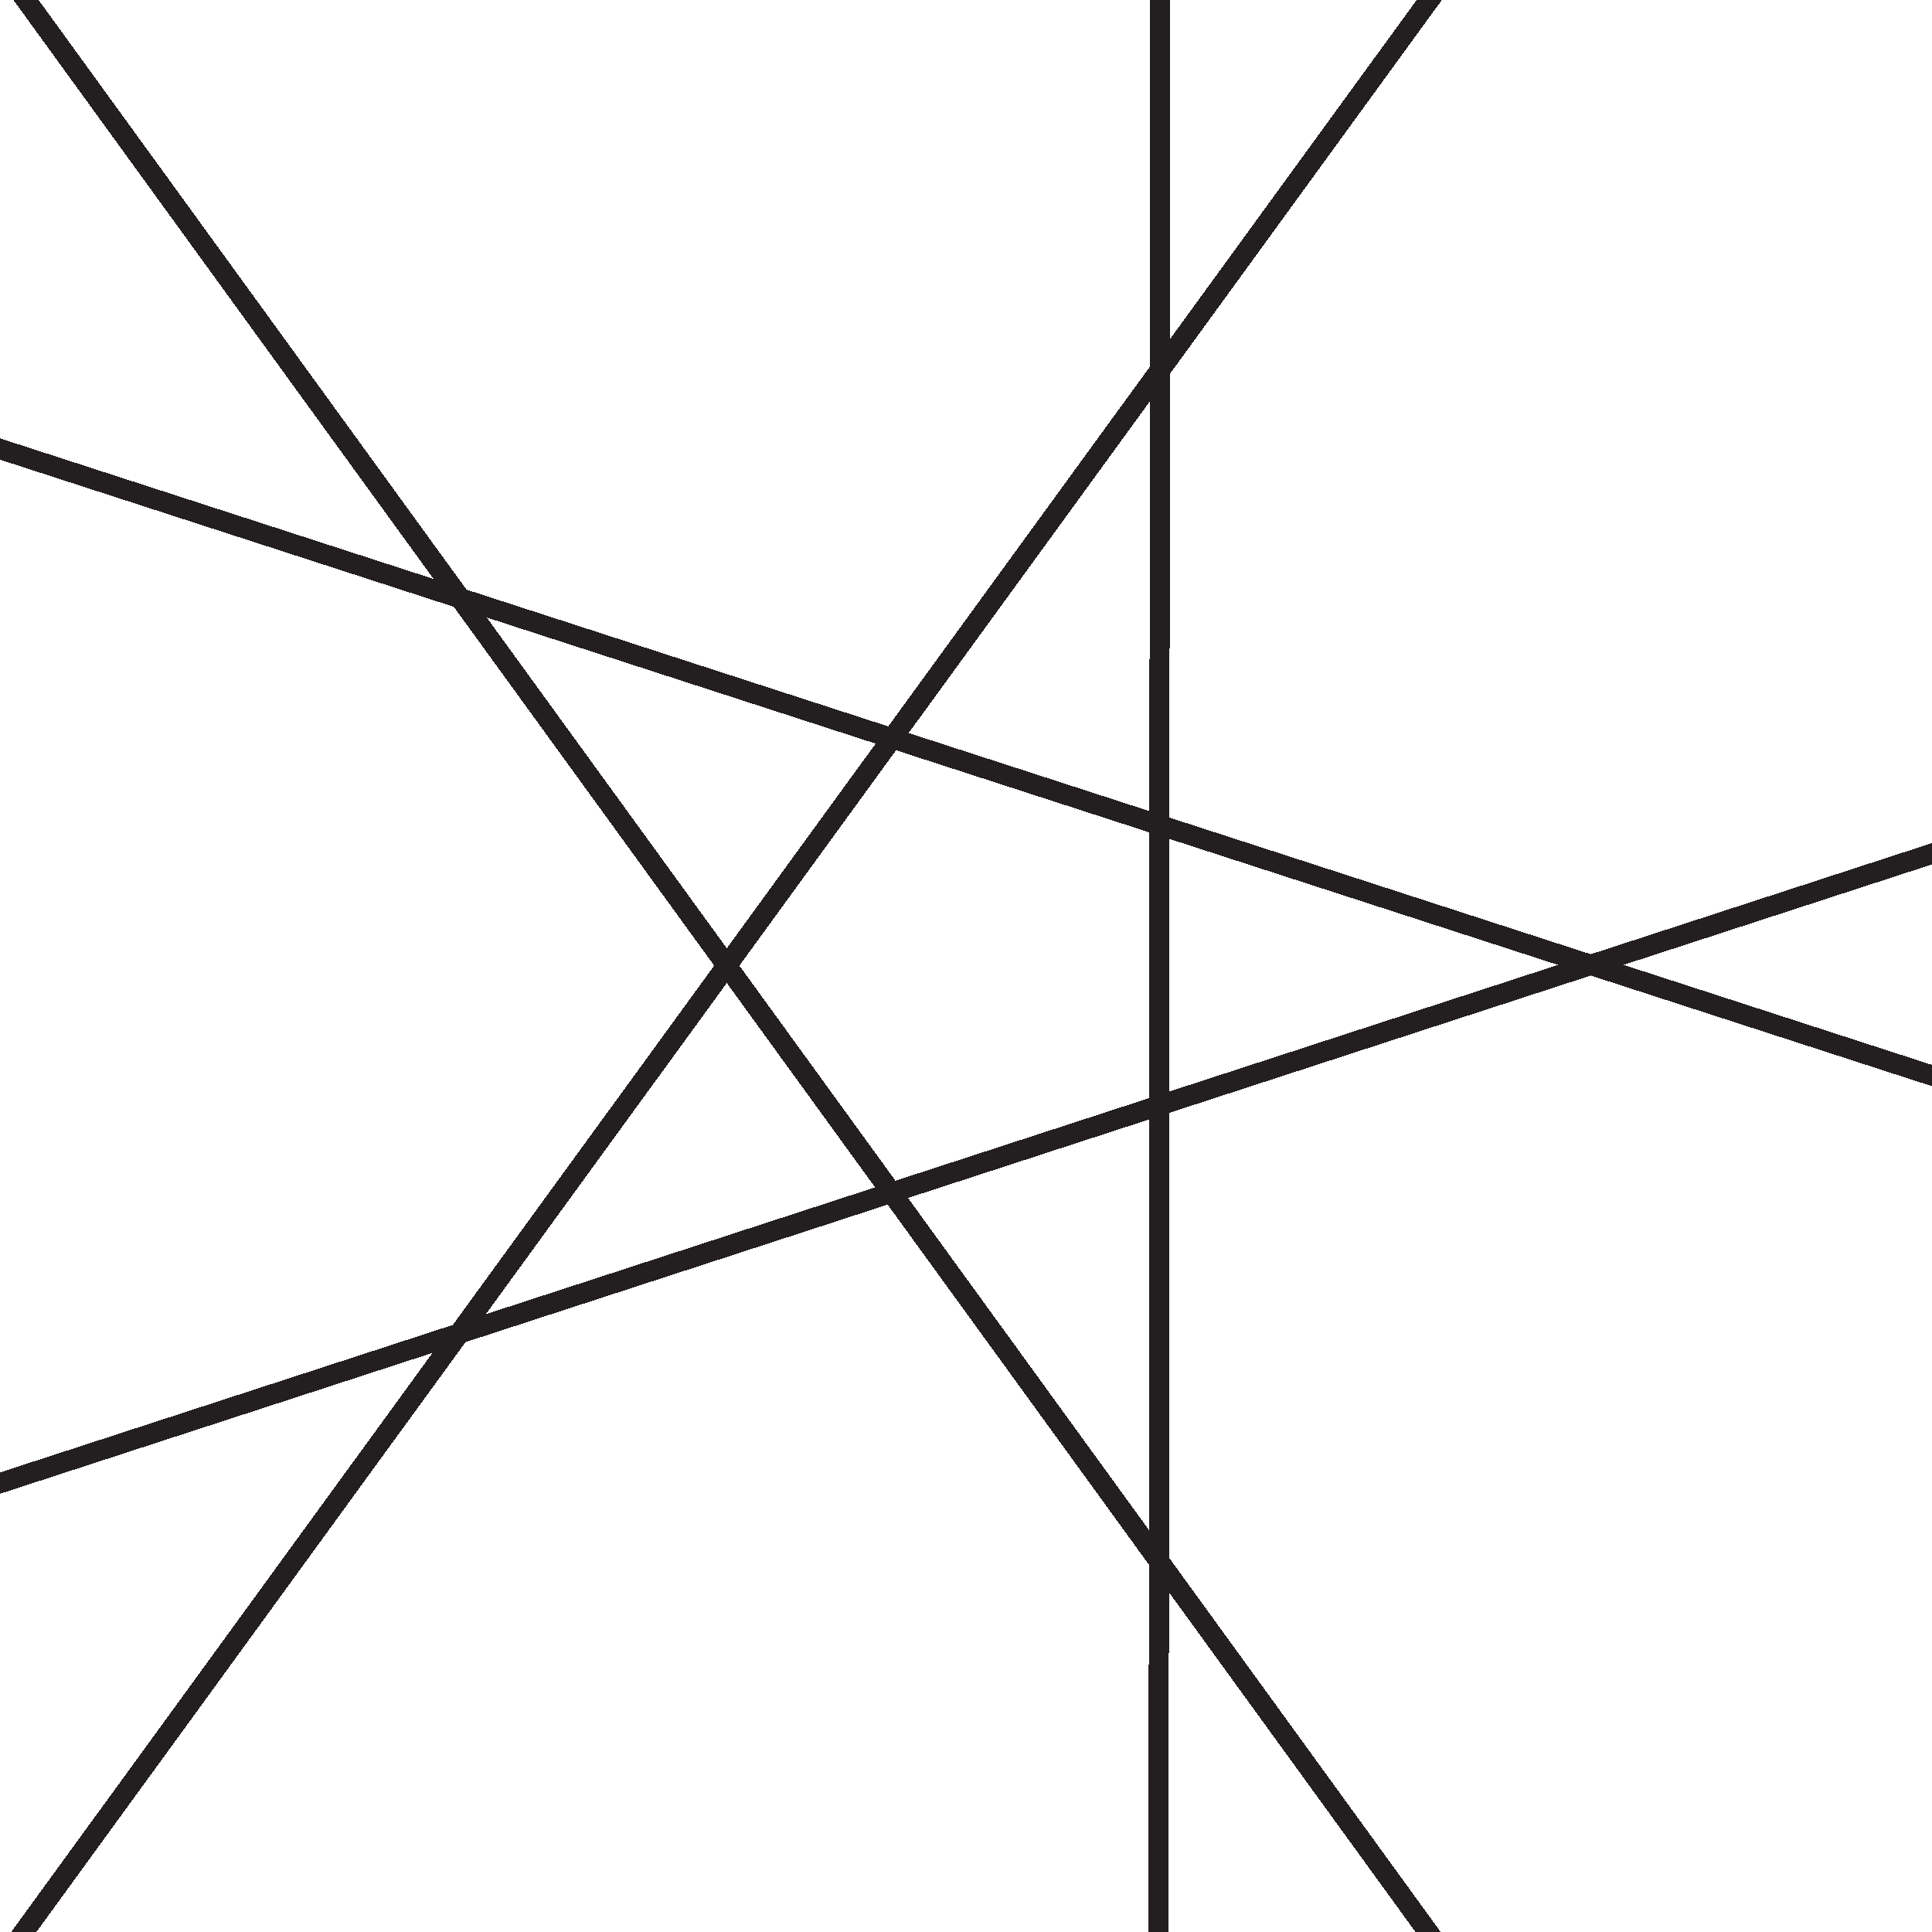
\includegraphics[height=1.2cm]{./../../common/images/rp5.pdf}
      \end{tabular}
    \end{center}
    \vspace*{-0.3em}    
    
    המשוואה של משטח זה היא 
    $S_5(x,y) + t(z)=0,$
    כאשר $S_5(x,y)$ הוא מחומש משוכלל (התמונה מימין) ו-$t(z)$ הוא
    גרסה של פולינומי צֶ'בישֶב שאותם כבר הזכרנו כאן במספר
    הזדמנויות.

     משטח נוסף ממעלה חמישית (משמאל) עם $15$ חודים נבנה על-ידי
    וולף בארת' (Wolf Barth); הוא קשור למשטח ממעלה רביעית של קלֶבּש (Clebsch; מימין) כפי שניתן לראות
    בתמונה האמצעית:

    \vspace*{-0.3em}
    \begin{center}
      \begin{tabular}{c@{\quad}c@{\quad}c}
        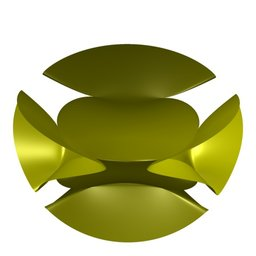
\includegraphics[height=1.2cm]{./../../common/images/barthquintic_green}
        &
        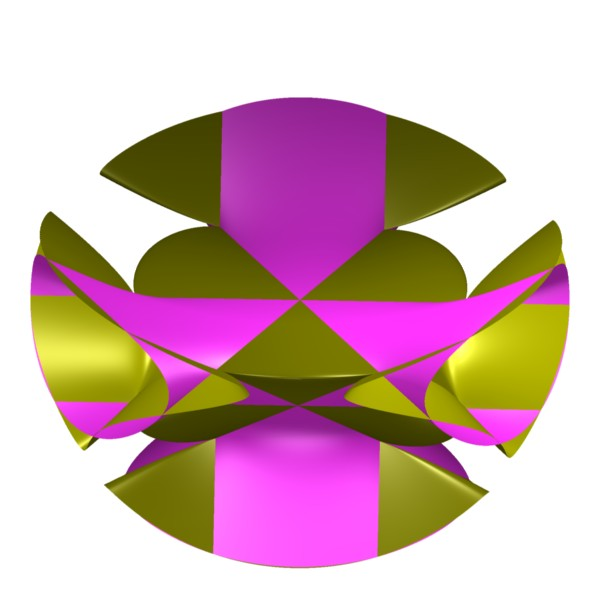
\includegraphics[height=1.2cm]{./../../common/images/barthquintic_clebschcubic}
        &
        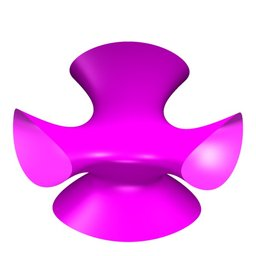
\includegraphics[height=1.2cm]{./../../common/images/clebschcubic_pink}
      \end{tabular}
    \end{center}
    \vspace*{-0.3em}
\end{surferPage}
